\section{Materials}

	All solvents were purchased from Sigma-Aldrich and used without any additional treatment.
	
	\Acr{fai}, \acr{mabr} MABr and \acr{mai} were either synthesized in-house (see page \pageref{methods-MAI}) or bought from GreatCell Solar.
	
	\PbItwo (99~\%), \PbBrtwo (99.999~\%), \CsI (99.999~\%), anhydrous chlorobenzene, anhydrous \gls{dmf}, and anhydrous \gls{dmso} were bought form Sigma-Aldrich and kept in a nitrogen-filled glovebox.
	
	Titanium(IV) isopropoxide (97~\%), acetylacetone, and \glsdesc{litfsi} (\gls{litfsi}) were bought from Sigma-Aldrich.
	
	4-tert-butylpyridine and hydroiodic acid 57~m/m\% in water were bought from Sigma-Aldrich and kept in a fridge (the colour of both these reagents change with ageing when kept out of the fridge).
	
	Spiro-OMeTAD was bought from 1-Material and stored in a nitrogen-filled glovebox.
	
	Methylamine in methanol (40~w/w\%, ca. 9.8~M) was bought from Tokyo Chemical Industry.
	
	\Gls{tae1}, \gls{tae3}, and \gls{tae4} molecules were used as received from Inés García-Benito, Agustín Molina-Ontoria and Nazario Martín (IMDEA, Madrid). The synthesis of \gls{tae1} has been described in \authoryear{Cabau2015a} and \authoryear{Choi2015b}. The synthesis of \gls{tae3} and \gls{tae4} has been described in CITATION.

\section{Synthesis, handling and purification}

	\subsection{\Acr{mai} synthesis}\label{methods-MAI}
	
		%Reference in laboratory notebook: [ig15, ig18, ig31, ig83].
		
		The synthetic method was inspired by \cite{Im2011a, Aharon2014, Williams2014, Etgar2012a, Nagaoka2015}.
		
		In a \SI{500}{\ml} one-necked flask (a big vessel helps later for drying) opened at air, \SI{14}{\ml} of a methylamine in methanol (40~w/w\%, ca. 9.8~M) were introduced. Dropwise, \SI{15}{\ml} of hydroiodic acid in water (57~m/m\%) was added while stirring and cooling at \SI{0}{\celsius}. This mixture was left stirring at room temperature and then still overnight covering the flask neck without completely closing it.
		The solution was evaporated in a vacuum-assisted rotatory evaporator at \SI{60}{\celsius}.
		The obtained white solid was scraped and transferred on a funnel with membrane filter (Sartorius, PTFE). It was washed with diethyl ether and the diethyl ether discarded. The solid was dissolved with ethanol, using as little volume as possible and vacuum was used for forcing the ethanol through the filter. The solid was recrystallized pouring abundant diethyl ether, then filtered, washed with diethyl ether and dried at vacuum overnight.

	\subsection{Lead salts handling}
		
		 Lead iodide and bromide bottles have to be opened in a nitrogen-filled glovebox. The failure in keeping the lead containing precursors away from oxygen seems to cause the formation of some lead oxide, a remaining non-soluble solid in the precursors solution which would have to be filtered away.
		 
	\subsection{Dense titania precursors solution}\label{dense-tio2}
		
		The precursors solution for the dense \TiOtwo layer was prepared using \SI{0.65}{\ml} of titanium(IV) isopropoxide and
		\SI{0.38}{\ml} of acetylacetone (strongly exothermic, add dropwise) in \SI{5}{\ml} of ethanol. The solution can be used just for a few days after preparation. Some hydrolysed product can be present in the solution, so it has to be filtered (PTFE, \SI{0.2}{\um}) just before the usage. The reader should consider the more stable and commercial precursor titanium diisopropoxide bis(acetylacetonate) as a convenient alternative.

	\subsection{CsFAMAPbIBr perovskite precursors solution}
		
		In a nitrogen-filled glovebox, \SI{507}{\mg} of \PbItwo, \SI{73.4}{\mg} of \PbBrtwo, \SI{172}{\mg} of \acr{fai} and \SI{22.4}{\mg} of \acr{mabr} were weighted and mixed in a \SI{5}{\ml} vial. For reducing the effect of static charging to the weighting process in the glovebox, a stainless steel weighing boat was fabricated. Already at this phase some reactivity can be seen between the mixed solids (lead based perovskites are known to be possible to synthesize in a mechanosynthesis solid-solid fashion), nevertheless this mixture can be stored in the glovebox for weeks without any sign of degradation.
		
		The same day of usage, \SI{0.2}{\ml} of anhydrous \gls{dmso} and \SI{0.8}{\ml} of anhydrous \gls{dmf} were added to the solid mixture of precursors. The solution was vigorously stirred at \gls{rt} for 1 hour. Heating or storing the solution for days has been observed to result in a yellow perovskite layer when deposited and annealed, so some kind of detrimental transformation is evident to happen in the solution, avoiding its storage for long time. Finally \SI{42}{\ml} of
		a \SI{1.5}{\Molar} \CsI solution in \gls{dmso} were added to the previous solution. The solution was filtered (PTFE, \SI{0.2}{\um}) just before its usage: even if the solution looks clear it can contain solid particles.

	\subsection{\Gls{spiro} and other \acr{htm} solutions for bottom cathode cells}
	
		A solvent with additives mix was prepared adding \SI{197}{\umol} of 4-tert-butylpyridine (\SI{28.8}{\ul}) to \SI{1}{\ml} of anhydrous chlorobenzene, then \SI{32}{\umol} of \gls{litfsi} (\SI{9.1}{\mg}) were added. The presence of 4-tert-butylpyridine allows the solubility of \gls{litfsi} in chlorobenzene.
		
		\Glsdesc{spiro} (\gls{spiro}) \acr{htm} solution was prepared dissolving \SI{59.0}{\umol} of \gls{spiro} (\SI{72.3}{\mg}) in \SI{1}{\ml} of the aforementioned solvent with additives mix.

		Other \acr{htm} solutions for bottom cathode cells were prepared dissolving either \SI{29.5}{\umol} of \glsdesc{tae1} (\gls{tae1}, \SI{36.6}{\mg}), \SI{19.7}{\umol} of \glsdesc{tae3} (\gls{tae3}, \SI{24.4}{\mg}), or \SI{9.83}{\umol} of \glsdesc{tae4} (\gls{tae4}, \SI{12.1}{\mg}) in \SI{1}{\ml} of solvent with additives further diluted with chlorobenzene in a 1:1, 1:2, 1:5 ratio respectively, in order to preserve the \acr{htm} to additives molar ratio of the \gls{spiro} solution (roughly \SI{3}{eq} of 4-tert-butylpyridine and \SI{0.5}{eq} of \gls{litfsi}). The lower concentrations were used due to the lower solubility of these \acr{htm} as compared to \gls{spiro} one.

\section{Perovskite Solar Cells}

	The "top" or "bottom" naming refers to the cell orientation during fabrication, so the "bottom" layer is the one in contact with the glass substrate.

	\subsection{Top Cathode Perovskite Solar Cells}

		\subsubsection{Anode and HTM substrate preparation}
		
		\subsubsection{MAPI Perovskite Two Step Fabrication}
	
	\subsection{Bottom Cathode Perovskite Solar Cells}

	
		\subsubsection{Cathode and ETM substrate preparation}
			This process was performed in a class 7 clean room.
		
			Pre-patterned \SI[product-units = single]{1.5 x 1.5}{\cm} \gls{fto} coated glasses (TEC7, \SI{7}{\ohm\per\sq}, Pilkington	\gls{fto} glass, \SI{2.2}{\mm} thickness, Xinyan Technology Ltd) were employed as substrate. The substrates were cleaned (ultrasonication) in water with Hellmanex soap, then in water, and finally in isopropanol; dried rubbing with a dust free cloth (from Berkshire) and the organic residuals were removed with an UV/ozone treatment for 20 minutes.
			
			Dense (as opposed to mesoporous) \TiOtwo layer was deposited (static dispensing, \SI{80}{\ul}) from the solution described in page~\pageref{dense-tio2} by spin-coating at \SI{3000}{\rpm}, \SI{3000}{\rpm\per\s}, for \SI{60}{\s} (\SI{\approx30}{\nm}) over the previously cleaned \gls{fto}. Then
			the substrates were sintered at \SI{500}{\celsius} for \SI{30}{\minute} and subsequently immersed in a \SI{40}{\milli\Molar}
			TiCl 4 solution in 9~\% HCl at \SI{70}{\celsius} for \SI{30}{\minute}, cleaned with water, with isopropanol and
			calcined at \SI{500}{\celsius} for \SI{30}{\minute}.
			
 			The usage of a thicker glass as compared to the one used for top cathode cells and the usage of \gls{fto} in place of \gls{ito} (\gls{fto} absorbs more in the infrared region and is way rougher) are needed for resisting the high temperature processing of the titania layers.
 			
		\subsubsection{MAPICl Perovskite Two Step Fabrication}
		
		\subsubsection{CsFAMAPbIBr Perovskite One Step Fabrication}
		
			The perovskite and HTM deposition processes were performed in a nitrogen-filled glovebox
			while constantly purging with a nitrogen flow for reducing the \gls{dmf} and \gls{dmso} vapours concentration.
			
			Perovskite precursor solution was filtered (\SI{0.2}{\um}, PTFE)
			and deposited by spin-coating (\SI{80}{\ul}, static dispensing, first step \SI{1000}{\rpm}, \SI{1000}{\rpm\per\s}, \SI{10}{\s};
			second step \SI{6000}{\rpm}, \SI{1000}{\rpm\per\s}, \SI{20}{\s}; fast crystallization was induced dynamically
			dispensing \SI{50}{\ul} of chlorobenzene on the spinning substrate \SI{5}{\s} before the end of the second
			step) obtaining a \SI{500}{\nm} thick perovskite layer. The substrates were directly transferred from
			the spin coater to a hot plate and annealed at \SI{100}{\celsius} for \SI{60}{\minute}. 
		
		\subsubsection{\Acr{htm} and cathode deposition}
		
		The \acr{htm} solutions (\gls{spiro}, \gls{tae1}, \gls{tae3}, or \gls{tae4}) were filtered (\SI{0.2}{\um}, PTFE) and deposited by spin-coating
		onto the perovskite layer (\SI{60}{\ul}, static dispensing, \gls{spiro} at \SI{4000}{\rpm}, \SI{4000}{\rpm\per\s},
		for \SI{30}{\s}; \gls{tae1} and \gls{tae3} at \SI{2000}{\rpm}, \SI{2000}{\rpm\per\s}, for \SI{30}{\s}; \gls{tae4} at \SI{1000}{\rpm}, \SI{2000}{\rpm\per\s},
		for \SI{45}{\s}) and similar HTM thickness were obtained (~100 nm). In order to increase the
		oxidative doping of the HTMs, the devices were kept 1 hour in dark in a dry air chamber.
		Finally, 80 nm of gold was deposited by thermal evaporation in an ultra-high vacuum chamber
		(\SI{1e-9}{\bar}) using a shadow mask leading to 4 diodes for substrate each with an active area of
		9 mm 2 .

	\subsection{Handling and Preservation}
		In case of bottom cathode cells, the oxidation of the HTM has been proven to improve the PCE. The oxidation can be induced via a dopant, for example FK209 CITATION, or via oxygen exposure. The latter has to be performed in dark as a synergic light and oxygen contribution on the perovskite layer degradation has been reported CITATION. The oxygen can enter in direct contact with the perovskite layer due to permeability of the HTM; additionally, when a mesoporous ETM is used (e.g. titania) oxygen can diffuse rapidly through the partially infiltrated mesoporous structure. For this reason a cabinet has been modified adding of a constant dry air inlet and physically reducing the leaks of the opening door edges.
				
		\begin{figure}%[!hbtp]%
			\centering
			\begin{subfigure}[b]{0.45\textwidth}
				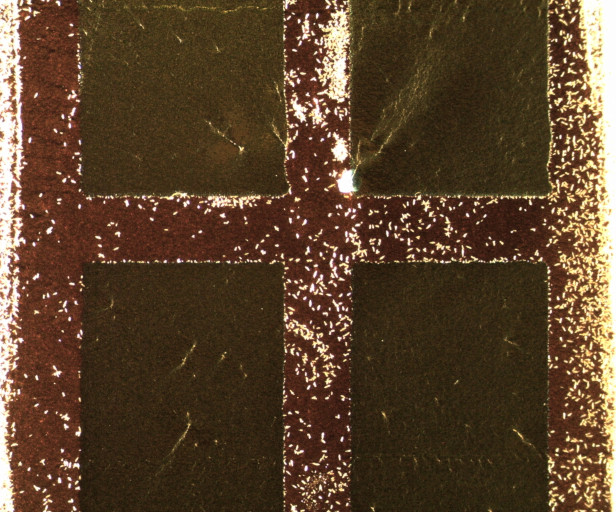
\includegraphics[width=1\textwidth]{microscope_degradation/ig93-1387-1-rescaled.jpg}
				\subcaption{Original cell, gold side.}\label{fig:microscope_degradation-start}
			\end{subfigure}
			\qquad
			\begin{subfigure}[b]{0.45\textwidth}
				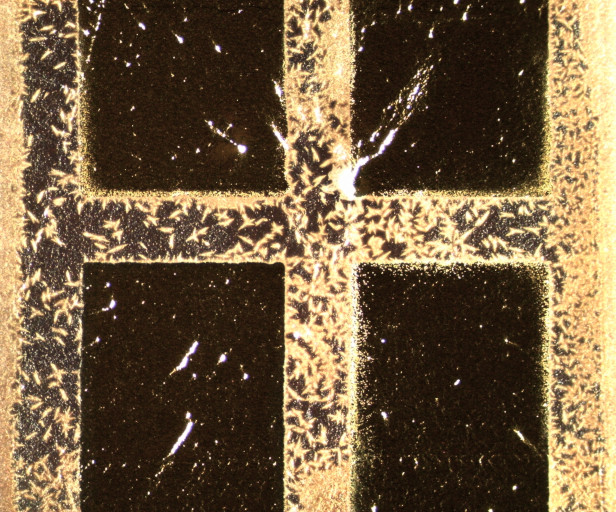
\includegraphics[width=1\textwidth]{microscope_degradation/ig93-1387-8-rescaled.jpg}
				\subcaption{After \SI{10}{\minute}, gold side.}\label{fig:microscope_degradation-end_front}
			\end{subfigure}
			\bigskip
			
			\begin{subfigure}[b]{0.45\textwidth}
				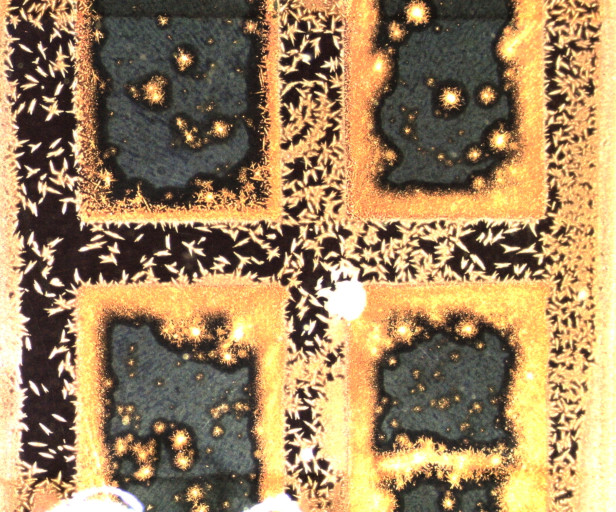
\includegraphics[width=1\textwidth]{microscope_degradation/ig93-1387-back-rescaled.jpg}
				\subcaption{After \SI{10}{\minute}, glass side.}\label{fig:microscope_degradation-end_back}
			\end{subfigure}
			\caption{Degradation of a \gls{fto}/\dTiOtwo/\mpTiOtwo/CsFAMAPbIBr/\gls{spiro}/Au device upon \SI{10}{\minute} illumination in air.}\label{fig:microscope_degradation}
		\end{figure}
	
		In Fig.~\ref{fig:microscope_degradation} the degradation of a complete device exposed to continuous illumination for 10 minutes and ambient air conditions is shown. An analogous device kept in air but without illumination did not show any degradation as observable via optical microscopy. The gold contact was not enough for protecting the perovskite layer from degradation, as oxygen could penetrate through the mesoporous titania. Interestingly the degradation is more prominent at metallic contacts' edges, one could speculate the reason being the electrical field being higher at smaller curvature metallic edges (seems that there's no therm in English for this, in Italian is referred as "effetto punta" and corona effect concentration ad edges derives from this). It could also be that the ionic profile of perovskite when holes quasi Fermi level is pinned at gold workfunction makes perovskite more sensible to degradation, and this is more evident at edges due to oxygen diffusion being blocked by the gold layer.

		Even if storage in dark and dry air should not be damaging for perovskite solar cells, the most usual long-term storage happens in a nitrogen-filled glovebox.

\section{Solar Cells Characterization}

	All the characterization on complete devices was performed keeping them in a air tight holder filled with nitrogen. The electrical connection from the cell electrode to the external end of the holder was obtained via gold tips connected via a printed circuit board to a coaxial cable.

	\subsection{Current-Voltage Curve}

		


	\subsection{Transient PhotoVoltage}
	
	\subsection{Charge Extraction}
	
	\subsection{Transient PhotoCurrent}
	
	\subsection{Differential Capacitance}
	
\section{Data Analysis and Handling}



